\appendix
\section{Housing Stock and Family Space}
\label{app:housing-stock}

This Appendix documents two facts about the housing stock that complement
the event study of Section~\ref{sec:empirical-evidence}: large homes are
mostly owned, and most large owned homes are held by older households.

\subsection{Large homes are owned}

Figure~\ref{fig:tenure-by-size} divides the 2023 housing stock in the
American Housing Survey (AHS) by number of bedrooms and tenure. Of the homes
with four or more bedrooms, 87 percent are owner-occupied and 9 percent are
rented. Of the homes with at most one bedroom, 13 percent are owner-occupied
and 74 percent are rented. In rooms, the unit of the rest of the paper, 43
percent of owner-occupied homes have seven or more rooms, against 7.5
percent of rented homes. The gap holds among families: owners with children
occupy 6.8 rooms on average and renters with children 5.2, and 48.7 percent
of renter households with children live in homes with at most two bedrooms,
against 7.4 percent of owner households with children. These shares describe
the homes households occupy rather than the homes on offer, but they show
that, in the existing stock, a family that wants a large home typically
buys one.

\begin{figure}[t]
\centering
\caption{Tenure of the Housing Stock by Number of Bedrooms (AHS 2023)}
\label{fig:tenure-by-size}
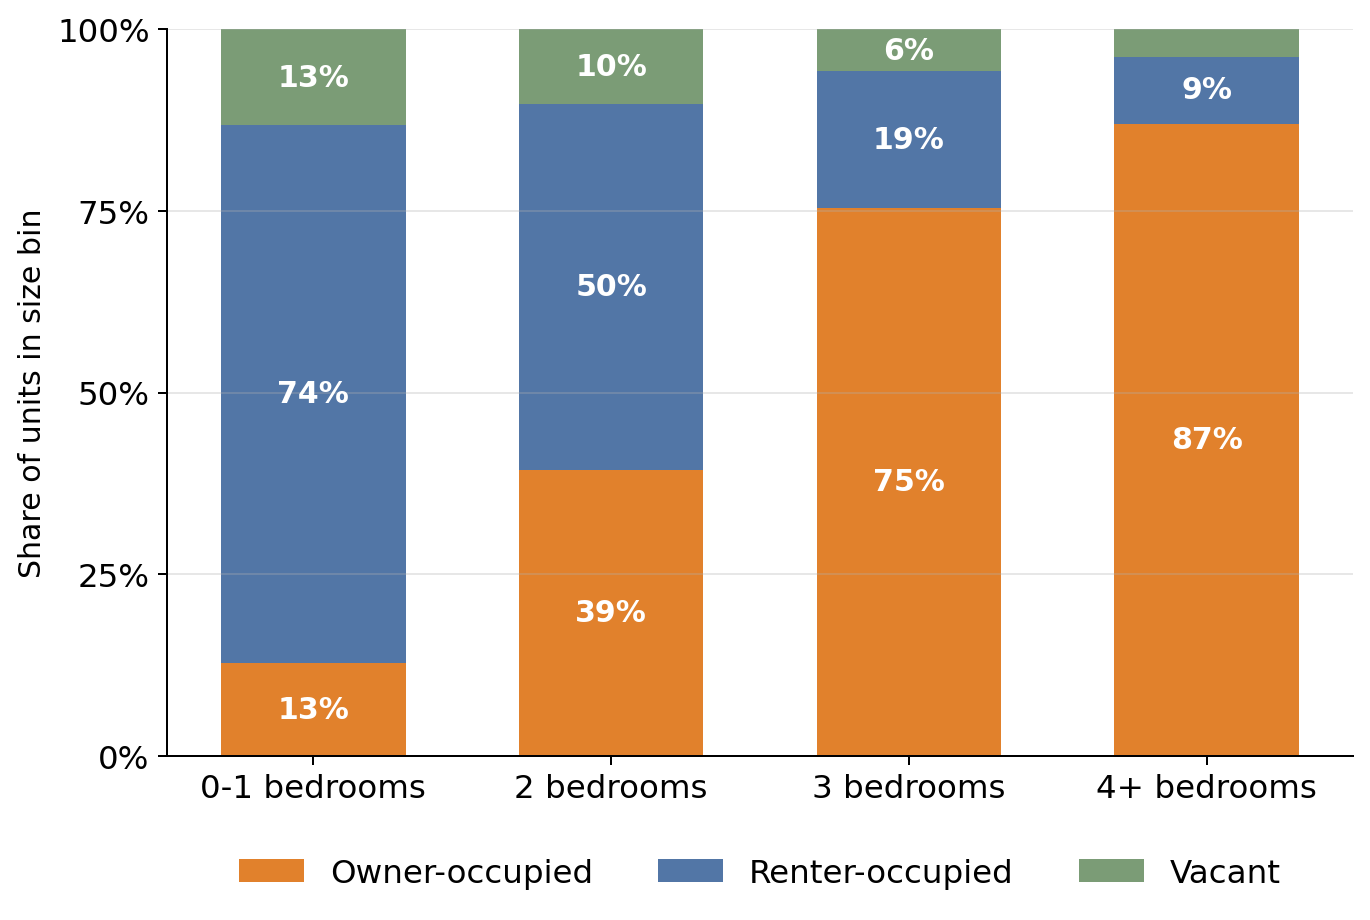
\includegraphics[width=0.62\linewidth]{ahs_tenure_share_within_size}
\par\medskip
\begin{minipage}{0.92\linewidth}
\footnotesize Note: This figure shows the tenure of housing units by number of
bedrooms. Each bar divides the housing units with the
stated number of bedrooms into owner-occupied units, units rented for cash,
and vacant units. Units occupied without payment of cash rent and units whose
occupants have a usual residence elsewhere are excluded. Weighted by the
housing-unit weight. Source: American Housing Survey 2023, national
public-use file.
\end{minipage}
\end{figure}

\subsection{Older households hold the large homes}

Figure~\ref{fig:large-homes} divides the owner-occupied homes with six or
more rooms in 42 large metropolitan areas in the 2023 American Community
Survey (ACS) by the age of the householder and by whether a child of the
householder younger than 18 lives in the home. Households aged 60 to 85
without children at home hold 40.0 percent of these homes, and households
aged 40 to 59 without children at home another 21.8 percent. Households aged
22 to 39 with children hold 10.6 percent. Across all ages, 68.3 percent of
the large owner-occupied homes house no child of the householder, close to
the 72.9 percent of all households in these areas without a child at home.
The large homes are therefore not held disproportionately by households
without children; they are held by the old. I call this concentration the
intergenerational allocation of housing. For a young family, it means that
the existing large homes become available mainly as older households sell
or leave them. The figure says nothing about the price at which older
owners would sell, or about whether young families would have more children
if they held these homes.

\begin{figure}[t]
\centering
\caption{Who Holds the Large Owner-Occupied Homes (ACS 2023)}
\label{fig:large-homes}
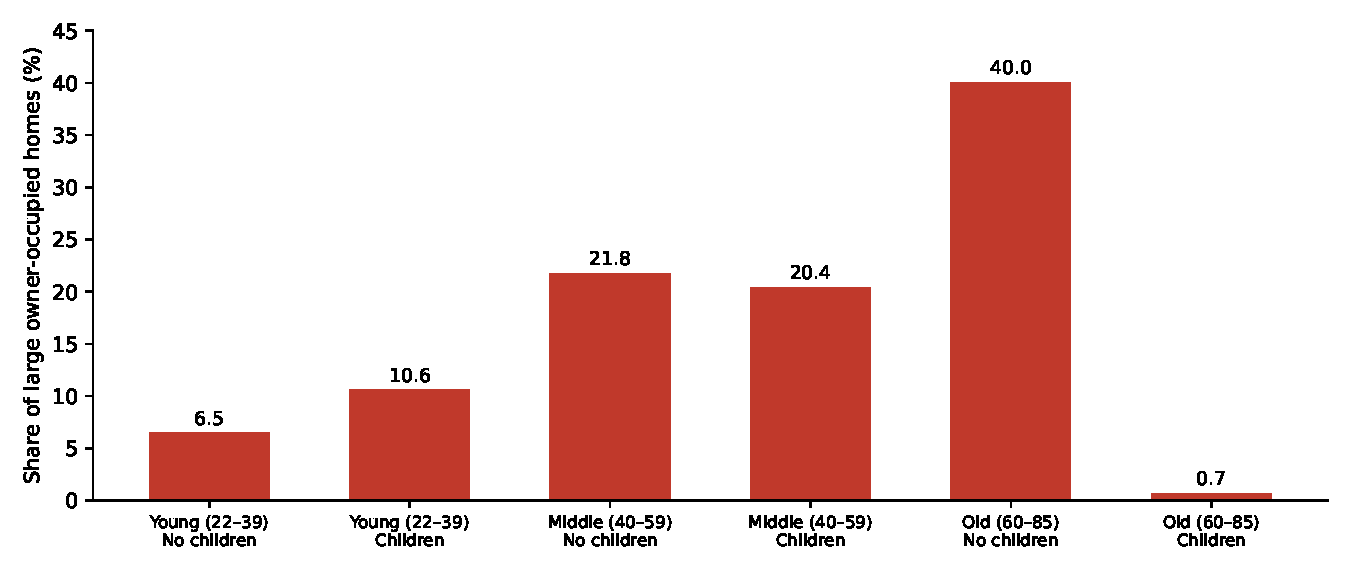
\includegraphics[width=0.9\linewidth]{large_homes_by_age_children_acs2023}
\par\medskip
\begin{minipage}{0.92\linewidth}
\footnotesize Note: This figure shows who holds the large owner-occupied
homes. Each bar is the share of owner-occupied homes
with six or more rooms held by households in the group; the six shares sum to
100 percent. Groups are defined by the age of the householder and by whether
an own child of the householder younger than 18 lives in the household.
Householders aged 22 to 85 in 42 large metropolitan areas, weighted by the
household weight; 289,109 households.
\end{minipage}
\end{figure}

\subsection{Ownership of recent parents}

The same pattern appears in the cross-section. In the 2005--2006 ACS,
household heads aged 30 to 55 whose oldest child is under four are 12.8
percentage points more likely to own than heads without children, a moment
the calibration also targets. Unlike the PSID estimates, this gap compares
different households at a point in time.

\subsection{Data}

The stock facts use the national public-use household file of the 2023
American Housing Survey, weighted by the housing-unit weight. Tenure has three
occupied categories: owned, rented for cash, and occupied without payment of
cash rent. Shares within a tenure use all units of that tenure as the
denominator; the share of seven-plus-room homes that are rented instead uses
all occupied units of that size. It is 8.2 percent when the denominator
contains owned and cash-rented units and 8.1 percent when it also contains
units occupied without cash rent and units with unreported tenure. Bedrooms and
total rooms are different measures. I report bedrooms for comparison with
other work and rooms because rooms are the PSID and ACS outcome and the unit of
the model. Mean rooms among households with children are computed over
households with at least one child present. A cross-section of occupied homes
does not identify the units offered for rent or the choices families would
make at other prices.


\section{Data and Empirical Measurement}
\label{app:empirical-data}

\subsection{PSID first-birth event studies}

\subsubsection*{Sample.}
The PSID data are the family and individual files for 1968--2023. An
observation is a person-year in which the person is a current member of a
family unit and at least 18 years old. The year of first birth is the earliest
birth year of a biological child in the person's relationship-to-child
history, which records up to twenty children. The comparison group consists of
persons whose full history reports no children; persons with incomplete or
unknown histories are dropped. A parent enters only if the first birth
occurs no earlier than the first year in which the person is observed as an
adult in the PSID. All estimates use the PSID longitudinal individual weight
and so include only sample persons with a positive weight.

The household sample keeps women who are the reference person or spouse of a
household containing a single current family unit, and keeps one woman per
household and year, the reference person first. The sample of adults heading a
household at baseline keeps treated adults, women and men, who were reference
person or spouse in the window two to three years before the first birth, and
retains all of their person-years. Eligible childless controls are retained
without this treated-sample restriction. The complementary sample keeps
treated adults who
were in the PSID but not reference person or spouse in that window. Each
sample compares first-time parents with eligible never-parents using the
same weights and entry rule. The main
text leads with the sample defined by household position before the birth,
which is also the sample definition used for the calibration's room-response
target. The other definitions show how the estimates depend on selecting a
household in the years around parenthood.

For the room response used in calibration, I further restrict observations
to the common support of the empirical panel and the model measurement
rules. This retains 112,148 person-years, 3,131 first-time parents and 5,954
childless controls. On this support, the room increase three to four years
after birth is 1.44 (standard error 0.05). The unrestricted baseline-head
sample gives 1.47 (0.05), as reported in the tables below. The difference is
the observation support, not a different event-time reference window or
birth definition. The tenure and moving regressions use their own available
observations and do not impose this room-specific restriction.
% Common support: output/model/first_birth_rooms_event_20261010/measurement_bridge/
% proposed_measurement_contract.json; original/rooms_coefficients.csv.
% Production use: output/model/production/2007/PROMOTION_RECEIPT_20261011_7p917.md.

\subsubsection*{Housing measures.}
All four housing items are taken from the official year-specific PSID family
variables and merged to the interview year in which they were reported. Rooms
are the total rooms in the dwelling except bathrooms, from the PSID question
``How many rooms do you have (for your family) not counting bathrooms?''. Codes that do not denote a count (9
through 1984; 99 in 1985--1993; 98 and 99 from 1994) are set to missing, and a
reported zero is retained. Ownership equals one if the family owns the
dwelling and zero if it rents; other arrangements are missing. The mobility
item asks whether the family moved since a fixed date: the spring of the
previous survey year in the annual waves, and January 1 of the previous survey
year in recent waves. It therefore records a move within an interval of about
one year in the annual waves and about two years in the biennial waves. The reason for a move is the first-mentioned
reason. ``More space'' is the PSID category for expansion of housing (more space,
more rent, a better place); ``neighborhood'' is the category for
neighborhood-related reasons (a better neighborhood, going to school, being
closer to friends or relatives). Unknown or unreported answers are missing, and code 9
of the reason item (unknown before 2019, homelessness in 2019) is treated as
missing throughout. An observation contributes to an outcome only when that
outcome is reported; unreported outcomes are never coded as zero.

% Source audit: the earlier merged panel placed housing on the preceding
% interview row: one year earlier through 1997 and two years afterwards.
% All 811,486 overlapping room values matched the following interview.
% The earlier 0.77-room estimate at year three compared rooms four to five
% years after birth with the year before or the year of birth.
Dating housing outcomes to the interview at which they are reported keeps
the outcome and first-birth clocks aligned.

\subsubsection*{Estimator.}
Event time is the survey year minus the year of first birth, grouped into the
windows $\le-8$, $-7/{-6}$, $-5/{-4}$, $-3/{-2}$, $-1/0$, $+1/{+2}$,
$+3/{+4}$, $+5/{+6}$, $+7/{+8}$, $+9/{+10}$ and $\ge+11$. Two-year windows
are needed because the PSID became biennial after 1997: from the 1999 birth
cohort on, no cohort is observed at both single years $-2$ and $+3$, so a
single-year reference period is observed for only part of the cohorts. The
omitted window is $-3/{-2}$, and each birth cohort must be observed in it;
cohorts without an observation in the reference window are excluded (first
births in 1968--1970 and 1985--1986 in the household sample, none in the
sample fixed at baseline). I estimate cohort-specific event paths relative to
the comparison group and average them with cohort-share weights, following \citet{sunAbrahamDynamicEffects2021}. The regressions include person and survey-year fixed
effects and complete sets of indicators for age and years of education.
Standard errors are clustered by person and account for the estimation of the
cohort shares.

\subsubsection*{Robustness.}
Table~\ref{tab:app-rooms-robust} collects alternative rooms estimates for the
sample of the main text. With the year before the birth in the reference
window ($-2/{-1}$), rooms are 1.12 higher two to three years after the birth.
Moving the reference window earlier gives 1.47 and 1.35 at three to four
years, because rooms change little before the birth in this sample; the
increase measured from years $-3/{-2}$ is 1.47, 1.47 and 1.42 across the
three reference windows. Using the harmonized room measure, aligned to the
interview at which it was reported, instead of the official year-specific
items changes the estimate by less than 0.01. Using the latest birth cohort
instead of the childless as comparison group leaves it unchanged. Requiring
the first birth to follow the first observation as reference person or spouse
does not bind in this sample, whose treated adults are reference person or
spouse two to three years before the birth.

\begin{table}[H]
\centering
\caption{Rooms Around the First Birth: Alternative Specifications (PSID)}
\label{tab:app-rooms-robust}
\footnotesize
\setlength{\tabcolsep}{4pt}
\begin{tabular}{@{}l cccccc@{}}
\toprule
 & (1) & (2) & (3) & (4) & (5) & (6) \\
 & Baseline & Reference & Reference & Reference & Harmonized & Latest cohort \\
 & & $-2/{-1}$ & $-5/{-4}$ & $-7/{-6}$ & room measure & as controls \\
\midrule
Change in rooms & 1.47$^{***}$ & 1.12$^{***}$ & 1.47$^{***}$ & 1.35$^{***}$ & 1.46$^{***}$ & 1.46$^{***}$ \\
 & (0.05) & (0.04) & (0.06) & (0.07) & (0.05) & (0.05) \\
Reference window & $-3/{-2}$ & $-2/{-1}$ & $-5/{-4}$ & $-7/{-6}$ & $-3/{-2}$ & $-3/{-2}$ \\
Reported window & $+3/{+4}$ & $+2/{+3}$ & $+3/{+4}$ & $+3/{+4}$ & $+3/{+4}$ & $+3/{+4}$ \\
Reference-window mean rooms & 4.69 & 4.87 & 4.81 & 5.06 & 4.70 & 4.69 \\
\addlinespace
\multicolumn{7}{@{}l}{\textit{Observations}} \\
N & 117,853 & 117,853 & 116,224 & 114,460 & 113,225 & 117,853 \\
N individuals & 9,310 & 9,310 & 9,263 & 9,205 & 9,235 & 9,310 \\
N first-time parents & 3,302 & 3,302 & 3,255 & 3,197 & 3,229 & 3,275 \\
\bottomrule
\end{tabular}
\par\smallskip
\begin{minipage}{0.97\linewidth}
\footnotesize Standard errors in parentheses. $^{+}$~$p<0.10$, $^{*}$~$p<0.05$, $^{**}$~$p<0.01$, $^{***}$~$p<0.001$.

\smallskip
Note: This table reports alternative estimates of the change in rooms around
the first birth for the sample of the main text: adults, women and men, who
were reference person or spouse two to three years before the birth. Column
(1) is the baseline of Table~\ref{tab:app-rooms-path}, column (2). Each other
column changes one element. Columns (2) to (4) move the reference window,
holding the sample fixed. Column (5) uses the harmonized room measure, aligned
to the interview at which it was reported, instead of the official
year-specific items. Column (6) uses the latest first-birth cohort as the
comparison group and keeps never-parents in the sample. ``Reference window''
is the omitted window and ``Reported window'' the reported one, both in years
relative to the first birth.
\end{minipage}
\end{table}

\subsection{ACS matched pseudo-panel}

The ACS exercise uses the one-year samples for 2005--2019 in all states and
the District of Columbia. The sample consists of women aged 25 to 45. Because
the ACS contains no birth histories, the year of first birth is inferred from
the age of the oldest child linked to the woman in the household roster, and a
woman's housing before that year is represented by childless women surveyed in
the corresponding earlier years who share her demographic matching cell.
Housing outcomes do not enter the matching. Rooms are capped at nine, and codes
that do not denote a count are missing; bedrooms are capped at five; ownership
equals one for owned units and zero for rented ones. The regression includes
event-time indicators from $-5$ to $+10$ with year $-2$ omitted, and state, age
and survey-year fixed effects; it is weighted by the matching weights, with
standard errors clustered by source household because a household can supply
several matched records. The estimation sample has 14.2 million matched
records from 2.8 million source households.

Between one year before and three years after the birth, rooms rise by 0.49
(0.01), bedrooms by 0.34 (0.004), and the ownership rate by 3.3 percentage
points (0.2). Dropping the age fixed effects, or all fixed effects, raises the
room estimate to 0.70 and 0.71 and the ownership estimate to 10.6 and 10.7
points; dropping the state and survey-year effects gives 0.53 rooms and 4.3
points. The pre-birth observations are constructed from other
women, so the design assumes that matched childless women represent the
housing future mothers would have had before the birth. The roster does not
record children living elsewhere or distinguish biological from other
children.

\subsection{Sibling-composition designs}

The ACS sibling designs use women aged 21 to 35 in the 2005--2019 one-year
samples whose oldest linked child, if any, is younger than 18. Children are
linked to mothers through the household roster, which records children living
with the mother, not all children borne, and does not separate biological from
step or adoptive children. The regressions control for complete sets of
indicators for the mother's age at the event, her race, the survey year and
the event age, are weighted by the person weight, and cluster standard errors
by household.

In the first design, the sample is mothers whose oldest linked child is aged 0
to 5 (857,607 mothers). The instrument indicates that the two oldest children
are recorded at the same age, and the treatment is a second resident child.
Ages are recorded in whole years without quarter of birth, so the instrument
is an age-only proxy for a twin birth. The first stage is 0.66 ($F$ statistic
above 77,000). The reduced form is 0.33 rooms (0.02), and the implied effect of
a second child is 0.50 rooms (95 percent interval 0.45 to 0.55), 0.33 bedrooms
(0.31 to 0.36), and 4.7 percentage points in ownership (3.3 to 6.1).

In the second design, the sample is mothers whose two oldest linked children
differ in age and whose second child is aged 0 to 5 (656,986 mothers); it is
not restricted to mothers with exactly two children. The instrument indicates
that the two oldest children have the same sex, and the treatment is a third
resident child. The first stage is 0.033 ($F=715$). Mothers of same-sex pairs
live in 0.038 fewer rooms (0.005) and 0.034 fewer bedrooms (0.003), and their
ownership rate does not differ. Scaled by the first stage, a third child would
reduce the dwelling by 1.15 rooms (95 percent interval 0.83 to 1.47). Children of the same sex can
share a bedroom, so sibling sex composition may change the space a family
needs without changing its size. That possibility would violate the exclusion
restriction for housing outcomes. The data cannot test it formally, and I do
not interpret this estimate as the effect of a third child. The same two designs are too imprecise in the PSID to add
information: same-age births are rare in its smaller sample, and the
sex-composition first stage is weak.

\subsection{Sample comparisons}
\label{app:empirical-two-samples}

Tables~\ref{tab:app-rooms-path} and \ref{tab:app-tenure-moves} compare two
sample definitions before imposing the calibration's common-support
restriction. The first keeps women who are reference persons or spouses in
each year. The second keeps treated adults, women and men, who held that position
two to three years before the birth and follows them thereafter; eligible
childless controls are retained. The second
is the household-position definition used in the main text. The room table's
1.47 estimate uses its full observation support, whereas the main-text room
figure and the calibration use the restricted-support estimate of 1.44.

Figures~\ref{fig:app-rooms-samples} and \ref{fig:app-tenure-samples} display
the paths under both definitions. Fixing household position before the birth
removes the pronounced pre-birth increase in rooms visible when the sample
is reselected in each interview. It also yields larger post-birth room and
ownership responses. The comparison makes household formation and sample
selection relevant to the measurement of housing around parenthood; it does
not isolate a causal effect of becoming a household head.

Both partners of a couple can appear in the sample. Clustering standard
errors by household instead of by person leaves the estimates unchanged
and raises the standard errors by at most 2.4\%.

\begin{figure}[p]
\centering
\caption{Rooms Around the First Birth, Two Samples (PSID)}
\label{fig:app-rooms-samples}
\includegraphics[width=0.9\linewidth]{first_birth_rooms_psid_samples}
\par\medskip
\begin{minipage}{0.92\linewidth}
\footnotesize Note: This figure shows the change in rooms around the first
birth for two samples: women selected as reference person or spouse in
each interview, and treated adults selected as reference person or spouse
before birth, with eligible childless controls. Both paths use the full sample for their definition and omit years
$-3$ and $-2$. The baseline-head path precedes the common-support restriction
used for the calibration target.
\end{minipage}
\end{figure}

\begin{figure}[p]
\centering
\caption{Ownership and Moving Around the First Birth, Two Samples (PSID)}
\label{fig:app-tenure-samples}
\includegraphics[width=0.95\linewidth]{first_birth_tenure_moves_psid_samples}
\par\medskip
\begin{minipage}{0.92\linewidth}
\footnotesize Note: This figure shows the change in ownership and moving for
the two sample definitions of
Figure~\ref{fig:app-rooms-samples}, using available observations for each
outcome. Reasons for moving in these panels are measured among all observed
households, rather than only among movers.
\end{minipage}
\end{figure}

\begin{table}[p]
\centering
\caption{Rooms Around the First Birth (PSID)}
\label{tab:app-rooms-path}
\small
\begin{tabular}{@{}l c c@{}}
\toprule
 & (1) & (2) \\
 & Women who are reference & Adults who were reference \\
 & person or spouse & person or spouse two to \\
 & in each year & three years before the birth \\
\midrule
\multicolumn{3}{@{}l}{\textit{Years relative to first birth}} \\
$-8$ or earlier & $-0.50$$^{***}$ & 0.15$^{+}$ \\
 & (0.12) & (0.08) \\
$-7$ and $-6$ & $-0.50$$^{***}$ & 0.04 \\
 & (0.10) & (0.06) \\
$-5$ and $-4$ & $-0.34$$^{***}$ & $-0.03$ \\
 & (0.06) & (0.04) \\
$-3$ and $-2$ & \multicolumn{2}{c}{reference window} \\
$-1$ and $0$ & 0.41$^{***}$ & 0.61$^{***}$ \\
 & (0.05) & (0.04) \\
$+1$ and $+2$ & 0.82$^{***}$ & 1.19$^{***}$ \\
 & (0.06) & (0.04) \\
$+3$ and $+4$ & 1.03$^{***}$ & 1.47$^{***}$ \\
 & (0.07) & (0.05) \\
$+5$ and $+6$ & 1.17$^{***}$ & 1.62$^{***}$ \\
 & (0.08) & (0.06) \\
$+7$ and $+8$ & 1.20$^{***}$ & 1.64$^{***}$ \\
 & (0.09) & (0.07) \\
$+9$ and $+10$ & 1.25$^{***}$ & 1.83$^{***}$ \\
 & (0.10) & (0.08) \\
$+11$ or later & 1.16$^{***}$ & 1.85$^{***}$ \\
 & (0.13) & (0.09) \\
\addlinespace
Reference-window mean rooms & 4.70 & 4.69 \\
\addlinespace
\multicolumn{3}{@{}l}{\textit{Observations}} \\
N & 63,338 & 117,853 \\
N individuals & 5,309 & 9,310 \\
N first-time parents & 3,655 & 3,302 \\
\bottomrule
\end{tabular}
\par\smallskip
\begin{minipage}{0.97\linewidth}
\footnotesize Standard errors in parentheses. $^{+}$~$p<0.10$, $^{*}$~$p<0.05$, $^{**}$~$p<0.01$, $^{***}$~$p<0.001$.

\smallskip
Note: This table reports interaction-weighted event-study estimates
\citep{sunAbrahamDynamicEffects2021} of the change in rooms relative to
years $-3$ and $-2$, in two-year windows of event time, with standard errors
clustered by person. The comparison group consists of adults with no children
in their full relationship history. All regressions include person and
survey-year fixed effects and indicators for age and years of education, and
use PSID longitudinal weights. Rooms are the total rooms in the dwelling
reported at the interview. Column (1) excludes first births in 1968--1970 and
1985--1986, which have no observation in the reference window. N individuals
counts first-time parents and childless controls.
\end{minipage}
\end{table}

\begin{table}[p]
\centering
\caption{Ownership and Moving Around the First Birth (PSID)}
\label{tab:app-tenure-moves}
\scriptsize
\setlength{\tabcolsep}{4pt}
\begin{tabular}{@{}l cccccc@{}}
\toprule
 & (1) & (2) & (3) & (4) & (5) & (6) \\
 & Owns the & Moved since & Moved for & Moved for & Share of moves & Share of moves \\
 & dwelling & last interview & more space & neighborhood & for more space & for neighborhood \\
\midrule
\multicolumn{7}{@{}l}{\textit{A. Women who are reference person or spouse in each year}} \\
$-1$ and $0$ & 0.11$^{***}$ & $-0.04$$^{**}$ & 0.014 & $-0.004$ & 0.054$^{**}$ & $-0.017$ \\
 & (0.01) & (0.02) & (0.009) & (0.006) & (0.017) & (0.012) \\
$+1$ and $+2$ & 0.16$^{***}$ & $-0.12$$^{***}$ & 0.034$^{***}$ & $-0.005$ & 0.140$^{***}$ & $-0.011$ \\
 & (0.02) & (0.02) & (0.009) & (0.006) & (0.021) & (0.014) \\
$+3$ and $+4$ & 0.16$^{***}$ & $-0.16$$^{***}$ & 0.020$^{*}$ & $-0.010$$^{+}$ & 0.133$^{***}$ & $-0.017$ \\
 & (0.02) & (0.02) & (0.010) & (0.005) & (0.023) & (0.014) \\
$+5$ and $+6$ & 0.14$^{***}$ & $-0.16$$^{***}$ & 0.007 & 0.002 & 0.108$^{***}$ & 0.022 \\
 & (0.02) & (0.02) & (0.010) & (0.006) & (0.026) & (0.018) \\
Reference-window mean & 0.41 & 0.58 & 0.070 & 0.032 & 0.122 & 0.054 \\
N & 61,229 & 63,817 & 62,813 & 62,813 & 19,456 & 19,456 \\
N individuals & 5,238 & 5,315 & 5,282 & 5,282 & 4,327 & 4,327 \\
N first-time parents & 3,619 & 3,656 & 3,640 & 3,640 & 3,105 & 3,105 \\
\addlinespace
\multicolumn{7}{@{}l}{\textit{B. Adults who were reference person or spouse two to three years before the birth}} \\
$-1$ and $0$ & 0.16$^{***}$ & $-0.07$$^{***}$ & 0.015$^{*}$ & $-0.009$$^{*}$ & 0.050$^{***}$ & $-0.022$$^{**}$ \\
 & (0.01) & (0.01) & (0.006) & (0.004) & (0.013) & (0.009) \\
$+1$ and $+2$ & 0.25$^{***}$ & $-0.17$$^{***}$ & 0.021$^{***}$ & $-0.008$$^{*}$ & 0.114$^{***}$ & 0.005 \\
 & (0.01) & (0.01) & (0.006) & (0.004) & (0.017) & (0.011) \\
$+3$ and $+4$ & 0.27$^{***}$ & $-0.21$$^{***}$ & 0.010 & $-0.009$$^{**}$ & 0.142$^{***}$ & $-0.002$ \\
 & (0.01) & (0.01) & (0.006) & (0.004) & (0.020) & (0.013) \\
$+5$ and $+6$ & 0.26$^{***}$ & $-0.21$$^{***}$ & 0.009 & $-0.003$ & 0.147$^{***}$ & 0.012 \\
 & (0.01) & (0.01) & (0.006) & (0.004) & (0.022) & (0.015) \\
Reference-window mean & 0.43 & 0.54 & 0.064 & 0.030 & 0.123 & 0.058 \\
N & 111,272 & 118,875 & 116,697 & 116,697 & 27,462 & 27,462 \\
N individuals & 9,070 & 9,346 & 9,245 & 9,245 & 5,488 & 5,488 \\
N first-time parents & 3,142 & 3,323 & 3,255 & 3,255 & 2,184 & 2,184 \\
\bottomrule
\end{tabular}
\par\smallskip
\begin{minipage}{0.97\linewidth}
\footnotesize Standard errors in parentheses. $^{+}$~$p<0.10$, $^{*}$~$p<0.05$, $^{**}$~$p<0.01$, $^{***}$~$p<0.001$.

\smallskip
Note: This table reports the change in ownership and moving in windows of
years relative to the first birth, relative to years $-3$ and $-2$, with the
same estimator, comparison group, controls, weights and reference window as
Table~\ref{tab:app-rooms-path}. The reference-window mean is the weighted mean
among first-time parents in years $-3$ and $-2$. Each outcome uses its own
sample of non-missing observations. ``Moved for more space'' equals one if the
household moved since the previous interview and gave expansion of housing (more space, more rent, a better place) as the
first reason, and zero otherwise; ``moved for neighborhood'' is defined in the
same way for neighborhood-related reasons (a better neighborhood, going to
school, being closer to friends or relatives). Columns (5) and (6) restrict
the sample to household-years with a move and therefore condition on an
outcome of the birth.
\end{minipage}
\end{table}

\begin{figure}[p]
\centering
\caption{Housing Outcomes by Years Relative to the First Birth (PSID)}
\label{fig:app-baselines}
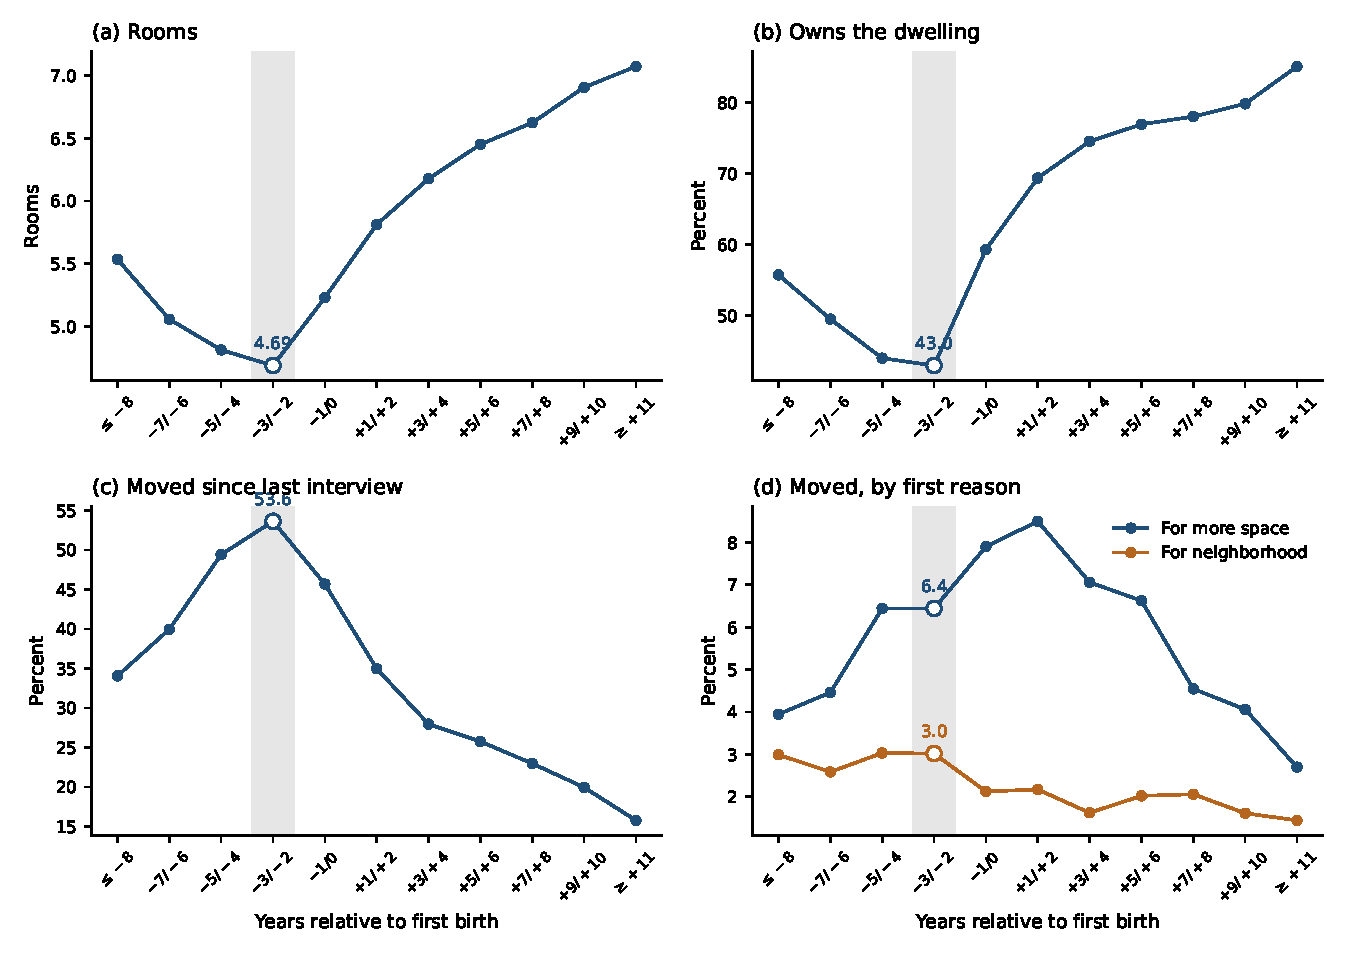
\includegraphics[width=0.95\linewidth]{figures/first_birth_baselines_A2h.pdf}
\par\medskip
\begin{minipage}{0.92\linewidth}
\footnotesize Note: This figure shows the levels of the housing outcomes
among first-time parents by two-year window of years relative to the first
birth, weighted by the PSID longitudinal weight. The sample is the one of
panel B of Table~\ref{tab:app-tenure-moves}: adults, women and men, who were
reference person or spouse two to three years before the birth. Each outcome
uses its available observations. The hollow marker and the shaded band mark
the reference window, years $-3$ and $-2$, and the label gives its level.
Levels are raw means, without fixed effects or controls; before the reference
window, these adults need not be reference person or spouse.
\end{minipage}
\end{figure}

\subsection{House value around the first birth}
\label{app:house-value}

The rise in rooms could reflect a move to a cheaper location, where space
costs less, rather than a larger expenditure on housing. To check this, I
estimate equation~\eqref{eq:event-study} for the log of house value, the log
of rooms and the log of house value per room among owners, and for a move
across state lines among all households. House values are reported by the
household and expressed in 2022 dollars. Table~\ref{tab:app-house-value}
reports the estimates three to four years after the birth. Among households
that already owned in the reference window, house value rises by 30 percent
and rooms by 17 percent, so value per room rises by 11 percent. The
coefficients on value per room before the reference window are small and not
significant. Moves across state lines become less frequent after the birth.
Households therefore do not obtain space by moving to places where it is
cheaper. Value per room reflects both location and the quality of the home,
so the estimates do not rule out a move to a suburb with similar prices per
room.

\begin{table}[H]
\centering
\caption{House Value Around the First Birth (PSID)}
\label{tab:app-house-value}
\footnotesize
\setlength{\tabcolsep}{4pt}
\begin{tabular}{@{}l ccccccc@{}}
\toprule
 & \multicolumn{3}{c}{All owners} & \multicolumn{3}{c}{Owners in $-3/{-2}$} & All households \\
\cmidrule(lr){2-4}\cmidrule(lr){5-7}\cmidrule(lr){8-8}
 & (1) & (2) & (3) & (4) & (5) & (6) & (7) \\
 & Log house & Log & Log value & Log house & Log & Log value & Moved across \\
 & value & rooms & per room & value & rooms & per room & state lines \\
\midrule
Years $+3$ and $+4$ & 0.230$^{***}$ & 0.146$^{***}$ & 0.084$^{***}$ & 0.265$^{***}$ & 0.157$^{***}$ & 0.108$^{***}$ & $-0.021$$^{**}$ \\
 & (0.024) & (0.011) & (0.021) & (0.025) & (0.012) & (0.023) & (0.007) \\
Reference-window mean & 228.3 & 5.96 & 38.9 & 228.4 & 5.94 & 39.3 & 0.089 \\
\addlinespace
\multicolumn{8}{@{}l}{\textit{Observations}} \\
N & 65,498 & 65,498 & 65,498 & 44,320 & 44,320 & 44,320 & 112,027 \\
N individuals & 6,501 & 6,501 & 6,501 & 4,712 & 4,712 & 4,712 & 8,961 \\
N first-time parents & 2,831 & 2,831 & 2,831 & 1,042 & 1,042 & 1,042 & 3,282 \\
\bottomrule
\end{tabular}
\par\smallskip
\begin{minipage}{0.97\linewidth}
\footnotesize Standard errors in parentheses. $^{+}$~$p<0.10$, $^{*}$~$p<0.05$, $^{**}$~$p<0.01$, $^{***}$~$p<0.001$.

\smallskip
Note: This table reports estimates of $\beta_k$ in
equation~\eqref{eq:event-study-weights} for the window three to four years
after the first birth, relative to two to three years before it. Sample,
estimator, weights and clustering as in Figure~\ref{fig:emp-rooms-own},
without the common-support restriction. Columns (1) to (6) keep owners with a
positive house value and rooms; columns (4) to (6) keep first-time parents who
owned at every interview two to three years before the birth. Each outcome
uses its available observations. The reference-window mean is the weighted
level among first-time parents in years $-3$ and $-2$: house value and value
per room in thousands of 2022 dollars, rooms, and the share moving across
state lines. A move across state lines compares the state of residence with
the previous interview, one or two years earlier.
\end{minipage}
\end{table}
